\chapter{State of the Art}\label{chapter:sota}
This chapter presents the state of the art (SotA) regarding approaches for GDPR compliance.
The first section (\autoref{sec:sota:models}) presents an overview of technological approaches for legal compliance to date.
The second section (\autoref{sec:sota:gdpr-semweb}) presents an overview of approaches for GDPR compliance utilising semantic web, with the third section (\autoref{sec:sota:gdpr-other}) presenting other approaches for GDPR compliance,
while the fourth section (\autoref{sec:sota:other}) presents approaches regarding regulatory compliance which do not directly concern the GDPR but are relevant towards understanding the SotA.
The chapter concludes (\autoref{sec:sota:analysis}) with an analysis of presented approaches and a discussion on the identified gaps for further work in the domain of utilising semantic web for GDPR compliance.

\section{Overview of Technological Approaches for Legal Compliance}\label{sec:sota:models}
This section provides an overview of technological approaches utilised for addressing legal compliance. It presents the different methodologies and frameworks for interpreting requirements from legal documents, and using technological frameworks towards the management of information and compliance.
To that end, the section utilises surveys and key publications in the last decade (2007-2019) to identify the state of the art.

\subsection{Classification of Approaches}
% 1> surveys of high level approaches to legal compliance
A survey of approaches within the last 50 years (from 2007) for addressing legal requirements \cite{otto_addressing_2007} provides the following categorisation:
\begin{itemize}
    \item \textbf{symbolic or mathematical logic}:  This approach attempts to balance use of natural language in legal documents with symbolic logic in an attempt to avoid ambiguities in interpretation. One of the earliest approaches, it was the precursor to later representations for machine and human readability.
    \item \textbf{knowledge representation}: This approach attempts to represent legal text as computer programs or algorithms by using logic programming techniques, primarily using Prolog, to avoid ambiguities in interpretation. The approach has been applied only within rigid domains where the law has minimal changes and does not rely on case law for interpretation. Additionally, the approach requires manual construction of logic rules from legal text, which prevents traceability. These challenges have limited its application to areas requiring requirements for system design, such as in software.
	\item \textbf{deontic logic}: This is another logic-based approach which involves capturing the rights and obligations provided within the law. The approach can be extending from representing this information to utilising it for preparing and assessing of compliance. This provides the necessary requirements which can be utilised in the development of business processes for legal compliance. Deontic logic has also been utilised to represent licensing and agreement requirements similar to those as legal text \cite{pellegrini_genealogy_2018}, and continues to be a topic of research in the areas of legal compliance \cite{palmirani_pronto:_2018,agarwal_legislative_2018,vos_odrl_2019}.
	\item \textbf{defeasible logic}: This approach consists of formulating rules of different types, namely - strict rules, defeasible rules, and defeaters - in order to represent the normative requirements extracted from legal text. Within the approach, strict rules must always hold, while defeasible rules hole true unless countered by an exception of a defeater. The approach is promised to provide better representation of conflicts in legal text in terms of interpretation as well as governance and jurisdiction requirements.
	\item \textbf{first order temporal logic}: This approach is based on using first-order temporal logic to extract key concepts such as - context, roles, type of information - and constructing logic-based requirements from those. The approach has not seen a large amount of interest, with existing applications limited to the privacy domain, and utilised for assessing compliance between privacy policies and laws.
	\item \textbf{access control }: Access control techniques have been utilised to capture the privacy-related elements of legal texts in the form of conditions and obligations that must be incorporated into a system as normative requirements for access to information. Conditions and obligations that cannot be represented as access control rules are incorporated as external environmental flags within the requirements. Utilising access control provides compliance by design, with logging providing transparency and accountability in the process. A survey of access control approaches utilising semantic web \cite{kirrane_access_2016} provides an overview of its applicability for different domains, including privacy enforcement.
	\item \textbf{markup-based representations}: This approach involves representing the hierarchical structure of legal text using markup-based representations such as SGML and XML. The representation enables the annotation of legal text and addition of metadata pertaining to definitions, acronyms, and citations. It also enables associating information about compliance requirements as well as interpretation. The United Nations and European Commission utilise this approach in publication of legislations and case law through standardised ontologies  \cite{palmirani_akoma_2018,european_union_eli_2015,van_opijnen_european_2011}.
	\item \textbf{goal based modelling}: This approach involves extracting and representing goals, soft goals, tasks, resources, and social relationships and modelling obligations to represent relationships for actors, dependencies, trust, delegation, and goal refinement. 
	\item \textbf{reusable requirements catalogue}: This approach constructs reusable catalogue of legal requirements derived from legal texts which are then applied to development lifecycles to incorporate compliance into systems. The use of the catalogue enables uncovering ambiguities and inconsistencies through use, and the refinement of the approach over time. The approach has been applied regarding security and personal data protection.
\end{itemize}

The survey paper provides comments on the applicability as well as limitation of each approach, and  outlines the following requirements engineering objectives (prefix \textit{REO}) an approach must take with in legal contexts to support the analysis of regulatory texts for requirements specification, system design, and compliance monitoring:
\begin{enumerate}[label={\textit{REO.\theenumi}}]
    \item \textbf{Identification of relevant regulations}: Finding relevant laws for a given system or process requires understanding of both - the requirements of the process as well as the context of the law. In addition, incorporating case law provides further challenges regarding application of relevant laws to processes due to the specifics and interpretation of requirements involved.
    \item \textbf{Classification of regulations with metadata}: In view of the above, the regulations need to be annotated or associated with metadata which can be utilised to classify them. This has been achieved to some extent through the EuroVoc\footnote{\url{https://eur-lex.europa.eu/browse/eurovoc.html}} - which is used as a multilingual and multidisciplinary thesaurus in the publication of metadata associated with EU legislations. However, where EuroVoc provides metadata about the domain of the legislation, greater granularity is needed to identify relevant information such as concepts, use-cases, and roles within the legal text.
    \item \textbf{Prioritisation of regulations and exceptions}: The hierarchical structure of regulations as well as relation to other regulations in terms of exceptions as well as overlaps and contradictions  must be taken into account for developing requirements.
    \item \textbf{Management of evolving regulations and law}: Changes in regulations need to be assessed by comparing the regulations, understanding the changes in requirements, and their application to existing systems for compliance. This requires traceability between legislations and requirements.
    \item \textbf{Traceability between references and requirements}: From the above, it is necessary to provide traceability from any section or clause with a reference in the legislation to the legal text being referenced. This is required in order to enable understanding of derived requirements from such sections across legislations.
    \item \textbf{Data Dictionary and glossary to ensure consistency}: Regulatory compliance makes use of consistent definitions and terminology an important aspect of requirements engineering. These are represented in the form of a data dictionary for domain-specific definitions and acronyms, and are utilised to support the requirements engineering process in providing a unified glossary for specifications, design, and compliance. 
    \item \textbf{Semi-automated navigation and searching}: The legislation needs to be accessible in both machine-readable as well as human-understandable states so as to enable technological approaches such as information extraction, annotations, searching, and automation in traceability of related information.
    \item \textbf{Annotation of regulatory statements}: It must be possible to associate annotations or additional information to regulatory statements, for example, with clarification of ambiguities or relevant case laws. Additionally, such annotations are also useful in a requirements engineering process to record assumptions and interpretations, and their usage in systems and applications.
    \item \textbf{Queries comparing legal concepts and compliance}: Finally, it must be possible query for information both within the text of the regulation as well as its associated information in order to support disambiguation and auditing for compliance. 
    Queries can assist with identification and comparison of applicable regulations, and to assess whether a particular requirement derived from the regulation has been addressed with respect to its compliance.
\end{enumerate}

\subsubsection{Discussion}
While the survey paper does not explicitly mention or refer to the linked data principles \cite{bizer_linked_2011}, some of the above objectives are fulfilled by utilising them in a given approach. Namely, linked data and semantic web provide an interoperable representation based in standards which can be used to define the required metadata regarding legislations, as demonstrated by EuroVoc, which addresses \textit{REO.1}, \textit{REO.2}, and \textit{REO.6} to some extent.

The use of structured representation to define legislations for \textit{REO.3} and \textit{REO.7} is possible using XML and ontologies such as ELI and Akoma Ntoso. However, ELI does not currently offer a way to represent the hierarchical structure of regulations, such as representation of individual articles or clauses, though the European Commission's Publication Office has stated their intention to provide this feature in the future.
This also limits the applications of \textit{REO.4} and \textit{REO.5} which require the above representation.
For creation of glossaries from legal text, the requirements of \textit{REO.6} are addressed through existing efforts such as EuroVoc and Interactive Terminology for Europe\footnote{\url{https://iate.europa.eu/}} (IATE), which provide consistent use of terms across domains, though there are no mechanisms to derive definitions from legislations or common interpretations of terms.

Regarding annotations for \textit{REO.8}, there exist standards such as W3C's Web Annotations model\footnote{\url{https://www.w3.org/annotation/}}, which can be utilised to annotate documents in an interoperable format, though they are not intended nor directly applicable for use over legislations.
Limitations to this are a lack of structured representation with sufficient granularity, for example, to reference individual clauses of text within the document.
Querying, as required for \textit{REO.9}, is inherently dependant on the underlying information representation, though there are standards such as SQL and SPARQL which provide interoperability in the approach.

\subsection{Approaches based on business process representations}
The use of approaches utilising business process representations for compliance are summarised in two key surveys. The first \cite{fellmann_state---art_2014} relates to the use of business processes within different phases of compliance, while the second \cite{benyoucef_information_2015} analyses use of information artefacts in business processes for compliance.

\subsubsection{Business Processes and Phases of Compliance}
A survey of business process approaches \cite{fellmann_state---art_2014} uses the following hierarchy of 4 dimensions to categorise approaches:
\begin{itemize}
    \item \textbf{Scope}: This dimension relates to the scope in terms of representation of processes, and concerns classes such as order and occurrence, information, resource, time, and location which describe the planning and execution of a process.
    \item \textbf{Lifecycle Phase}: This dimension indicates the period in time addressed by the representation in terms of design (ex-ante,a-priori,ad-hoc), execution, and after execution (ex-post,a-posteriori,post-hoc). The approaches related to design representation focus on prevention of compliance adherence and avoiding violations by design, whereas those concerned with after execution are focused on demonstration of compliance and detection of violations. Approaches concerned with execution are focused on real-time observation and prevention of violations.
    \item \textbf{Formality}: This dimension categorises approaches as addressing compliance in terms of its verification and validation, or whether addressing business processes. The approaches addressing business processes are analysed in terms of their annotation and representation of information relevant to compliance, and categorised based on their formality in terms of whether they focus on formalisation, compliance checking, end-user oriented, management orientied, and is a framework or a method.
    \item \textbf{Contribution Type}: This dimension indicates whether the approach provides a technical artefact as an implementation, or a conceptual model checking method, with approaches not satisfying either criteria being categorised as `other'.
\end{itemize}

\subsubsection{Information Artefacts in Business Processes for Compliance}
A survey of information artefacts used in business processes for compliance \cite{benyoucef_information_2015} provides the following categories for artefacts based on their type and use. These artefacts are used by business process across all phases (ex-ante, execution, ex-post) of compliance and represent the different stages of compliance management.
\begin{itemize}
    \item \textbf{System design artefacts}: These artefacts provide structure or behaviour-related description of a system, through some formalism such as UML or text.
    \item \textbf{Method}: These artefacts provide definitions of activities to create or interact with a system.
    \item \textbf{Language or notation}: These artefacts are a formalised system for statements represents parts of reality.
    \item \textbf{Algorithm}: These artefacts provide executable descriptions of system behaviour.
    \item \textbf{Guideline}: These artefacts provide suggestion regarding behaviour in specific situations.
    \item \textbf{Requirements}: These artefacts provide statements about systems and their properties.
    \item \textbf{Pattern}: These artefacts provide definition of reusable elements of design with its benefits and application contexts.
    \item \textbf{Metric}: These artefacts provide a mathematical model able to measure aspects of systems or methods.
\end{itemize}
These artefacts are used for tasks associated with regulatory compliance, including enactment, analysis, checking, and modelling. The survey finds that existing approaches have over the years been largely focused on the modelling and checking tasks in the context of regulatory compliance, with compliance analysis being increasingly researched over time  while enactment has received little attention. The survey concludes that compliance approaches are basically limited to identifying relevant requirements from laws and regulations and ensuring that business processes comply with them, without much attention to compliance enactment.
This gap can be addressed by developing technologies for activities such as anticipation, adaptation and management of change to business processes as and when they occur.

\subsubsection*{Discussion}
The business processes are represented for organisational planning and management purposes using standard representations such as UML and BPMN. These can be reused for compliance management tasks by applying and assessing the compliance requirements over these processes. For this, it is necessary to align the business processes and the artefacts they use with the compliance requirements and terminology. The two approaches discussed in the earlier sections presented existing work in terms of categorising such approaches based on their use of business processes in phases of compliance, and the information artefacts they use. Through this, they provide the different avenues where an approach might assist with the compliance process, as well as the type of artefacts it might use to do so.

Depending on the context, such as - type of activities, legal requirements, use-case - one or more of the categories can be adopted for creating an approach for compliance. For example, the requirement of ensuring activities are compliant before they are executed in GDPR can be fulfilled by an approach utilising business process representations in the ex-ante lifecyle phase with the verification and validation being performed through any of the categorised information artefacts with varying degrees of formality. Assessing them purely from a compliance management perspective would serve to diminish their usefulness and prevalence in the planning and management of activities.

As legal requirements evolve, it could be a costly exercise to create and adopt a new approach to meet its compliance. Therefore, an evolving approach needs to identify and adapt the new compliance requirements over existing representations of business processes through development of validation and verification mechanisms.
This requires the business process representations to be in an form which can reused for such purposes, such as through the example of interoperable standards.

\subsection{Approaches utilising Legal Ontologies}
Surveys on legal ontologies provide categorisation of ontologies as well as their intended applications within the domain. One such survey \cite{rodrigues_legal_2019} categorises the purposes as - organising and structuring information, reasoning and problem solving, semantic indexing and searching, and understanding a domain. It also categorised them based on the generalisation of concepts as - upper level ontology, core ontology, domain ontology, and application ontology - with most of them falling under core and domain ontologies. The survey also provides an overview of the methodologies used, and the evaluation approaches utilised, which consist of - evaluation by specialists, data-driven evaluations, gold-standard assessments, application in case study, and those that have no evaluation or are unclear. The survey also shows that most ontologies are formalised using RDF/OWL-DL though other formalisations were also utilised.

Another survey\footnote{One of the analysed ontologies is GDPRtEXT, which is one of the major contributions of this thesis. The survey provides a comparison of GDPRtEXT with the SotA, and is described in more detail in \autoref{sec:voc:GDPRtEXT}.} \cite{leone_taking_2019} categorises ontologies in the five domains of - policies, licenses, tenders and procurement, privacy, and cross-domain. It then analyses the ontologies based on features such as the intended domain, purpose, year, license, development, source of concepts, base ontology, and formalism.

A survey of approaches capturing privacy requirements in the SotA \cite{gharib_towards_2017} identified and categorised concepts and relationships as agentive (actor, role), intentional (goal, action), informational (asset, information), interaction (delegation, permission, trust), risk (threat, vulnerability, attack), treatment (mitigate, constraint, policy), and privacy (requirement, notice, anonymity).
Another survey \cite{van_de_ven_qualitative_2016} categorises privacy policy languages based on their focus (machine, human, privacy, security), aspects (authorisation, spatial, temporal, law), and syntax (XML, high-level, logical).
Both surveys identify the gaps in the SotA in terms of absence or limitation of approaches to sufficiently express concepts, and propose an ontology to fill the gaps.
Further surveys represent the SotA in their respective areas regarding access control \cite{kirrane_access_2016}, rights expression languages \cite{pellegrini_genealogy_2018}, privacy policy languages \cite{van_de_ven_qualitative_2016}, privacy requirements engineering \cite{gharib_ontologies_2016}.

In areas of compliance, standardisation of representations for norms and requirements has seen efforts such as LegalRuleML \cite{palmirani_legalruleml:_2011} which uses temporal and defeasible logic, and has been applied for compliance checking over business processes \cite{governatori_semantic_2016}. On similar lines, Compliance Management Ontology \cite{syed_abdullah_compliance_2012} proposes shared conceptualisation of business process management, culture management, obligations, programme, resources, risk management, and solutions.

\subsubsection{Discussion}
Ontologies have been extensively used for formal representations of information, rules \cite{kirrane_scalable_2018}, rights \cite{pellegrini_genealogy_2018}, legislations \cite{leone_taking_2019}, business processes \cite{elgammal_formalizing_2016}, policies \cite{van_de_ven_qualitative_2016}, and requirements \cite{gharib_ontologies_2016}.
However, there has also been a noted lack of guidelines regarding their reuse, particularly within the legal domain for compliance \cite{casanovas_legal_2017}.
Within the legal domain, evaluation of developed ontologies is a challenge due to the requirement of specialists or legal experts being involved in the modelling stage \cite{rodrigues_legal_2019}.
Despite these hurdles, ontologies continue to be researched and utilised as a solution for assisting with the legal compliance.

The state of the art in ontologies thus presents encompassing representations for documents, requirements, rules, obligations, policies, and business processes associated with legal compliance. An adopter has a range of approaches to choose from based on the stated methodologies and formalisms, where the choice of approach depends on the stated requirements and goals of the ontology as well as its role in the legal compliance process.

\section{Approaches for GDPR compliance utilising Semantic Web}\label{sec:sota:gdpr-semweb}
\subsection{Research Projects utilising Semantic Web}

\subsubsection{SPECIAL}
SPECIAL\footnote{\url{https://www.specialprivacy.eu/}} (Scalable Policy-aware Linked Data Architecture For Privacy, Transparency and Compliance) is an European H2020 Project that aims to provide technical solutions for data protection requirements associated with use-cases involving big data. It features extensive use of semantic web technologies across a variety of compliance related tasks such as recording provenance logs of data processing \cite{kirrane_scalable_2018}, providing visual interfaces for consent \cite{drozd_consent_nodate,gritzalis_i_2019}, compliance checking of processing activities based on given consent \cite{westphal_spirit:_nodate,vos_odrl_2019,fernandez_user_2019}, and efforts towards standardisation of related vocabularies\footnote{The SPECIAL project was the primary driving force behind the creation of the W3C Data Privacy Vocabularies and Controls Community Group (DPVCG), of which the author was an active participating member. Information about this has been listed in \autoref{sec:intro:dpvcg}. The Data Privacy Vocabulary (DPV), produced by the DPVCG, has also been documented as a deliverable of the project in D6.5 \cite{pandit_d6.5_2019}.} \cite{pandit_creating_2019}.
Collaborations between SPECIAL and other projects have produced related work, such as an approach for compliance checking using ODRL \cite{agarwal_legislative_2018,vos_odrl_2019}, and the application of SPECIAL's framework in a Smart City use-case \cite{fernandez_user_2019}.
Information about the methodologies used, developed technologies, and their evaluations is accessible through peer-reviewed publications and public deliverables\footnote{\url{https://www.specialprivacy.eu/publications/public-deliverables}}.

SPECIAL uses a distributed ledger to store the processing logs for data processing activities, which can be evaluated for compliance against given consent in ex-ante and ex-post phases. The logs are stored using the  Policy Log vocabulary\cite{bonatti_special_2018-1} with the data processing activities represented by Usage vocabulary \cite{bonatti_special_2018-2}. Compliance evaluation is performed by using a custom reasoning algorithm \cite{bonatti_fast_2018} in a semantic reasoner. The consent is provided in a visual and interactive form to the user using the web browser \cite{drozd_consent_nodate,gritzalis_i_2019}. The project has been successfully applied to use-cases provided by its commercial partners\footnote{See D1.5 \cite{bonatti_d1.5_2018} and D1.6 \cite{schlehahn_d1.6_2018} for information on use-cases.} as well as in an external use-case related to use of IoT in Smart Cities \cite{fernandez_user_2019}. The Figure. \ref{fig:SPECIAL-architecture1} presents an overview of the SPECIAL architecture along with its components and utilised technologies.

\begin{figure}[htbp]
    \centering
    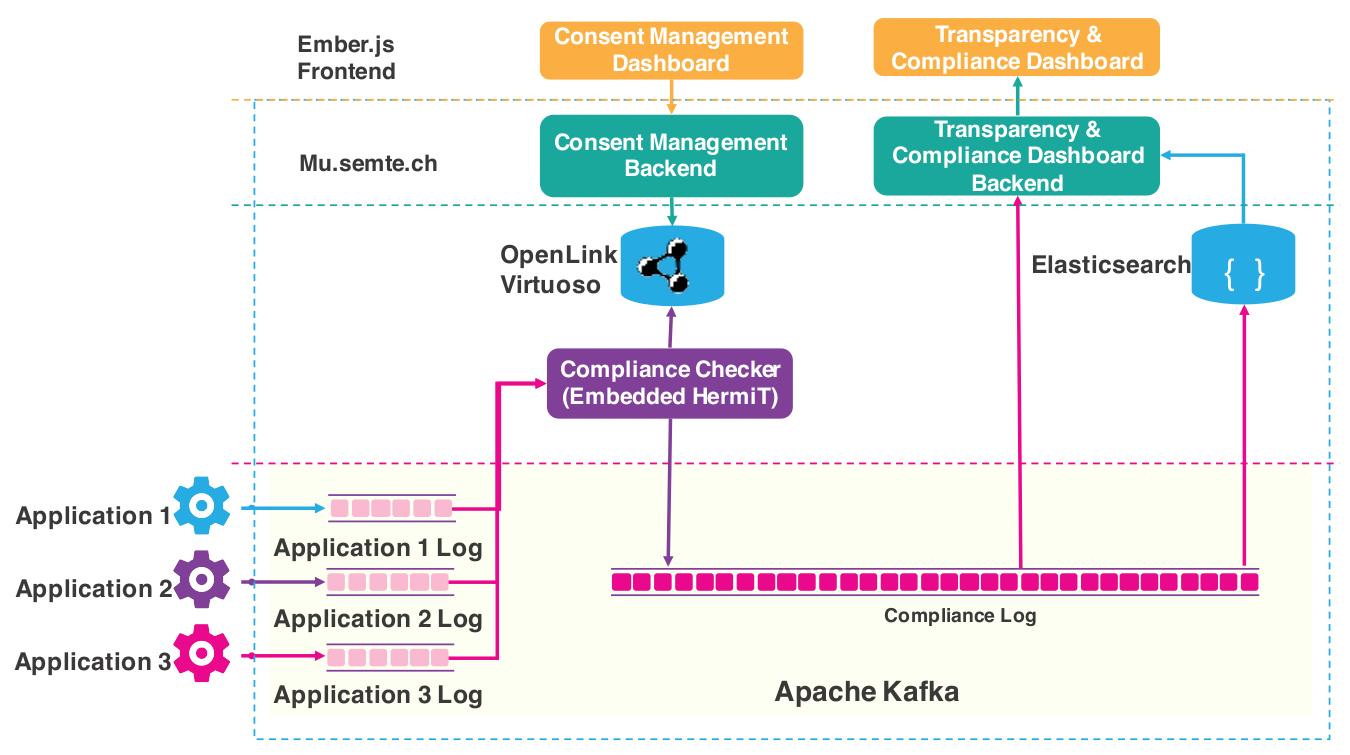
\includegraphics[width=\linewidth]{img/SPECIAL_architecture1.png}
    \caption{Overview of SPECIAL Architecture \cite{kirrane_scalable_2018}}
    \label{fig:SPECIAL-architecture1}
\end{figure}

The Usage Policy \cite{bonatti_special_2018-2} is used to represent data processing activities and is described in more detail in D2.5 \cite{bonatti_d2.5_2018}. The base policy uses OWL2 expressions to denote an intersection of personal data categories, processing operations, purposes, recipients, and storage. These can then be combined using OWL2 unions over multiple base policies with differing expressions. SPECIAL provides additional vocabularies for purposes, personal data categories, processing operations, and recipients for using with the Usage Policy based on its use-cases. The general form of a base policy is:
\begin{lstlisting}
ObjectIntersectionOf(
    ObjectSomeValuesFrom(spl:hasData SomeDataCategory)
    ObjectSomeValuesFrom(spl:hasProcessing SomeProcessing)
    ObjectSomeValuesFrom(spl:hasPurpose SomePurpose)
    ObjectSomeValuesFrom(spl:hasRecipient SomeRecipient)
    ObjectSomeValuesFrom(spl:hasStorage SomeStorage)
)
\end{lstlisting}
The storage expression is itself a policy comprising of OWL2 expressions specifying the storage location, duration, and interval. The general form of a storage policy is:
\begin{lstlisting}
ObjectIntersectionOf(
    ObjectSomeValuesFrom(spl:hasLocation SomeLocation)
    ObjectSomeValuesFrom(spl:hasDuration SomeDuration)
    DataSomeValuesFrom(spl:durationInDays Interval)
)
\end{lstlisting}

For a given policy $P_c$ representing activities permitted by given consent and policy $P_s$ representing processing activity, compliance is evaluated by checking whether $P_c$ complies with $P_s$ - which in OWL2 is checked by using a reasoner to check whether $P_c \subseteq P_s$. This is performed by using an algorithm \cite{bonatti_fast_2018} in a semantic reasoner that is optimised for speed by only performing those operations associated with checking for compliance between policies.

The activity is recorded in a log using the Policy Log vocabulary \cite{bonatti_special_2018-1}, represented in Figure. \ref{fig:SPECIAL-policy-log-vocabulary}, and is evaluated for compliance by using the reasoner in both ex-ante and ex-post phase. The Policy Log vocabulary, described in D2.7 \cite{kirrane_d2.7_2018}, reuses existing vocabularies such as DCAT and PROV \cite{lebo_prov-o:_2013}, and is used to record an immutable documentation of compliant activities and their legal basis in consent.

\begin{figure}[htbp]
    \centering
    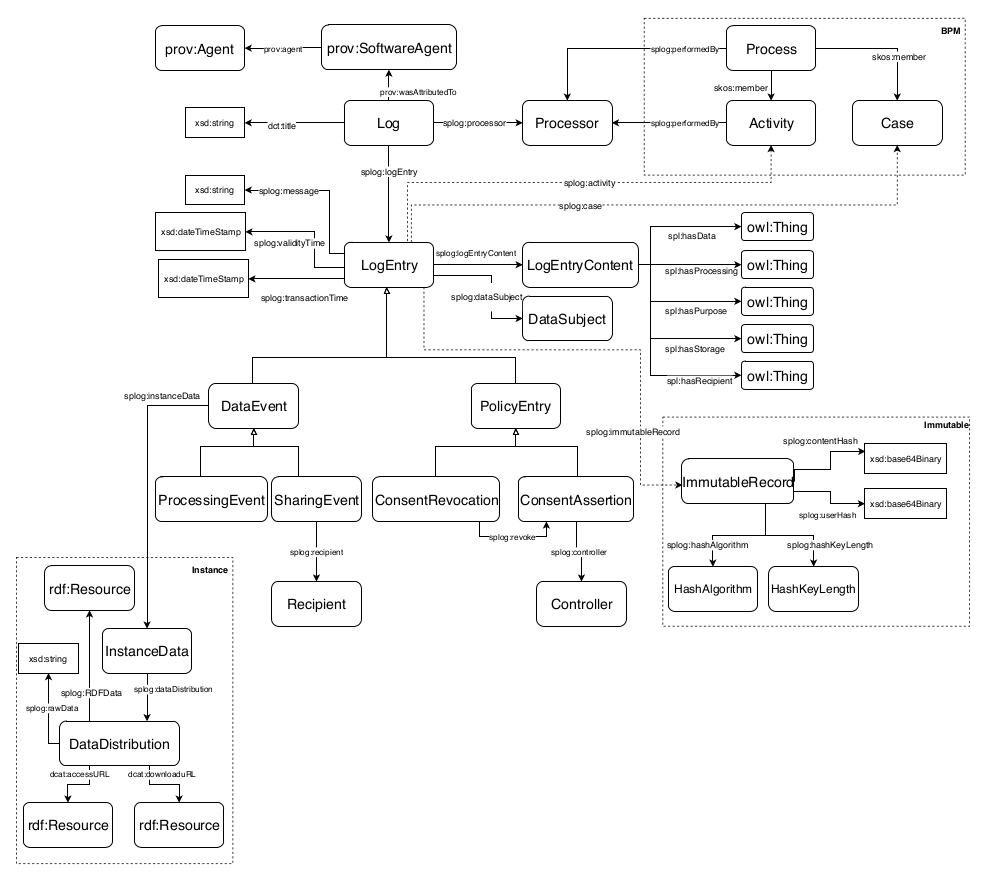
\includegraphics[width=\linewidth]{img/SPECIAL_logvocabulary.png}
    \caption{Overview of SPECIAL Policy Log Vocabulary \cite{bonatti_special_2018-1}}
    \label{fig:SPECIAL-policy-log-vocabulary}
\end{figure}

The methodologies associated with the vocabularies produced by the SPECIAL project are based on the utilisation of metadata in the compliance process \cite{wenning_compliance_2018}.

SPECIAL's work has also produced ODRL models for deontic representations of GDPR requirements through collaborations with other projects. The first of this is based on work with the Austrian SERAMIS\footnote{\url{https://cordis.europa.eu/project/rcn/189040/factsheet/en}} (Sensor-Enabled Real-World Awareness for Management Information Systems) project, which produced a web-based tool called PriWUcy for evaluating compliance assessments of GDPR articles \cite{agarwal_legislative_2018}.
The tool uses a model of the legislation created by parsing the legislation text and representing the obligations using ODRL. A set of preliminary assessment questions provides the inputs over which the model is applied to identify actions and obligations to be fulfilled as part of the assessment. The ODRL model, depicted in Figure. \ref{fig:SPECIAL-ODRL}, is extended to represent additional granularity of constraints of - Feature, Discretional, and Dispensation. The ODRL policies are associated with the text of the GDPR they represent through classes representing chapters, articles, and paragraphs within the text of the GDPR. The approach relies on identifying and representing assets, parties, actions, duties, and constraints using the developed ODRL model. More information on the tool can be found in the public deliverable D5.5 \cite{agarwal_d5.5_2017}.
\begin{figure}[htbp]
    \centering
    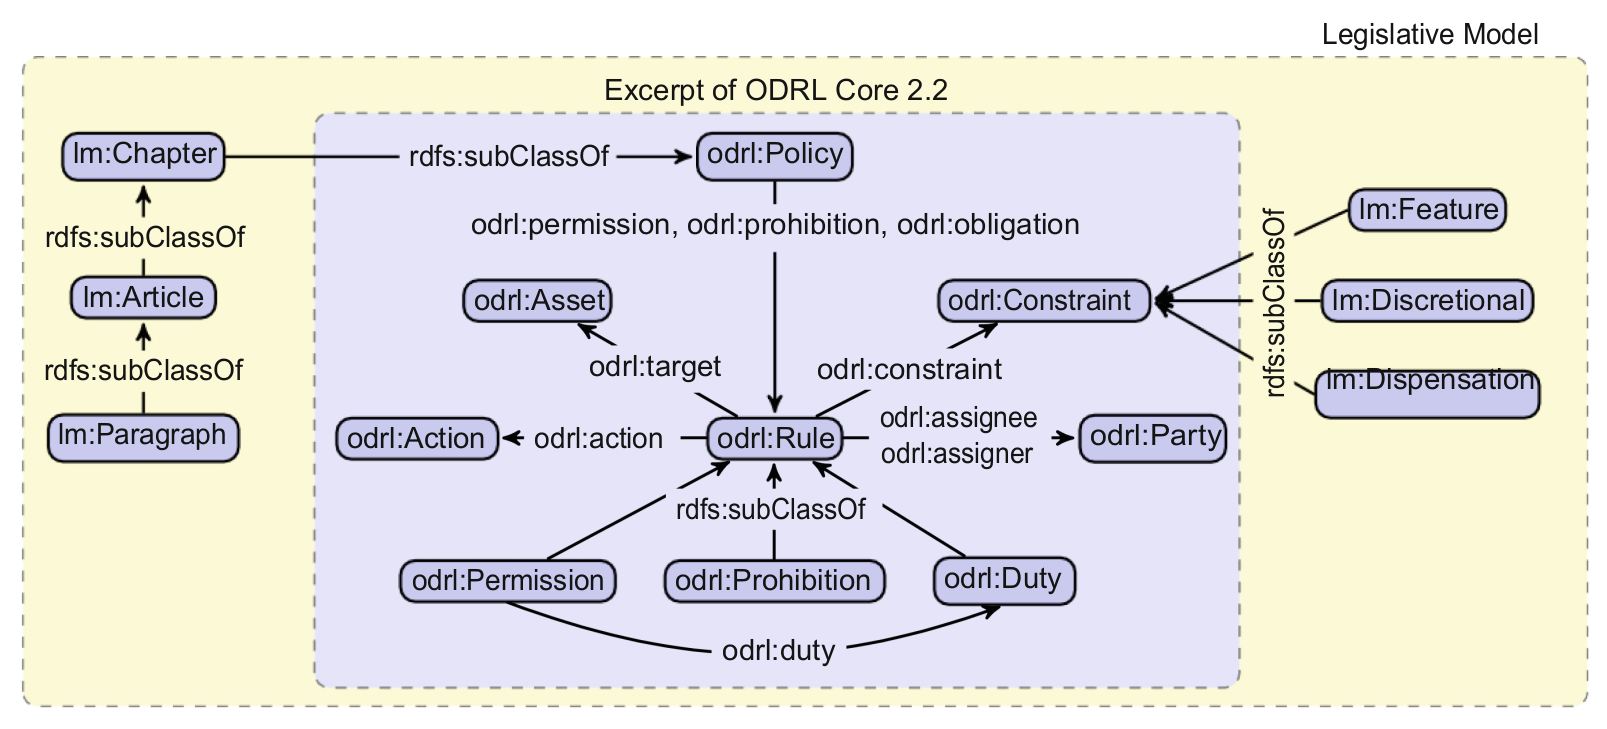
\includegraphics[width=\linewidth]{img/SPECIAL_ODRL.png}
    \caption{Extension of ODRL for representing GDPR obligations \cite{agarwal_legislative_2018}}
    \label{fig:SPECIAL-ODRL}
\end{figure}

The ODRL profile was further developed for modelling regulatory obligations and business policies based on GDPR towards compliance checking and providing explanations of the reasoning process \cite{vos_odrl_2019}. Additional classes and properties added include those relevant for specifying the legal bases, purpose, location, and safeguards associated with processing. Policies representing articles in the GDPR are checked against permissions by activities to perform a data processing operation. For example, the following listing shows a request for transfer personal data to a third country based on consent, which would be checked against the corresponding policy representing Article 46 of the GDPR. 
\begin{lstlisting}
<http://example.com/policy:bp-transfer> a orcp:Set ;
    odrl:profile <http://example.com/odrl:profile:regulatory-compliance> ;
    orcp:permission
    [ odrl:action orcp:Transfer ;
        orcp:data orcp:PersonalData ;
        orcp:responsibleParty orcp:Controller ;
        orcp:organisationType orcp:InternationalOrganisation ;
        orcp:sender <http://example.com/CompanyA_Ireland> ;
        orcp:recipient <http://example.com/CompanyA_US> ;
        orcp:recipientLocation orcp:ThirdCountry ;
        orcp:purpose orcp:PersonalRecommendations ;
        orcp:legalBasis orcp:Consent ;
        odrl:dataSubjectProvisions orcp:EnforceableDataSubjectRights ;
        odrl:dataSubjectProvisions orcp:LegalRemediesForDataSubjects
    ] .
\end{lstlisting}
Compliance is checked by converting the ODRL policies into InstAL, a domain-specific language for writing models based on events and states, which translates to Answer Set Programming (ASP) and is evaluated using a solver. When a policy is found to be non-compliant, explanations are generated based on `fluents' - facts that are true if present and false if absent - through a reasoning process. The implementation is publicly accessible through a hosted repository\footnote{\url{https://github.com/instsuite/instsuite.github.io/blob/master/gdpr.ial}}. An example of this is as follows:
\begin{lstlisting}
# fluents capturing justifications
type Article;
fluent permission(Subject,Article);
fluent prohibition(Subject,Article);
noninertial fluent supports(Subject,Article,Predicate,Object);
noninertial fluent lacks(Subject,Article,Predicate,Object);

# if enforceable data subject rights are defined, the term is true
article46_body_term2(Process) when
    triple(Process,dataSubjectProvisions,enforceableDataSubjectRights);
supports(Process,article46,dataSubjectProvisions,
        enforceableDataSubjectRights) when
    article46_body_term2(Process),
    triple(Process,dataSubjectProvisions,enforceableDataSubjectRights);

# otherwise the description lacks data, and non-inertial fluents are applied
lacks(Process,article46,dataSubjectProvisions,
        enforceableDataSubjectRights) when
    applies(Process,article46),
    not supports(Process,article46,dataSubjectPro
\end{lstlisting}

The second work is based on applying SPECIAL's GDPR compliance framework to the Austrian CitySPIN\footnote{\url{http://cityspin.net/}} (Cyber-Physical Social Systems for City-wide Infrastructures) project, which utilises linked data platforms to ingest data from multiple sources in a smart city scenario, and utilises it for data processing pipelines and analytics. An important component of the project is the management of consent which utilises SPECIAL's policies \cite{bonatti_special_2018-1,bonatti_special_2018-2} and compliance framework \cite{kirrane_scalable_2018}.
The auxiliary vocabularies provided by SPECIAL for purpose and data categories were extended for use-cases associated with CitySPIN \cite{fernandez_user_2019}, as depicted in Figure. \ref{fig:SPECIAL-CitySPIN}. 
The defined policies are checked in the ex-ante and ex-post phase using the SPECIAL compliance checking algorithm \cite{bonatti_fast_2018}, with a prototype implementation demonstrating ex-ante compliance checking in ad-hoc widgets sharing personal data \cite{fernandez_privacy-aware_2019}. Details about the project and its implementation are available through its public deliverables D6.1 \cite{noauthor_d6.1_nodate} and D6.3 \cite{noauthor_d6.3_nodate}.

\begin{figure}[h]
    \centering
    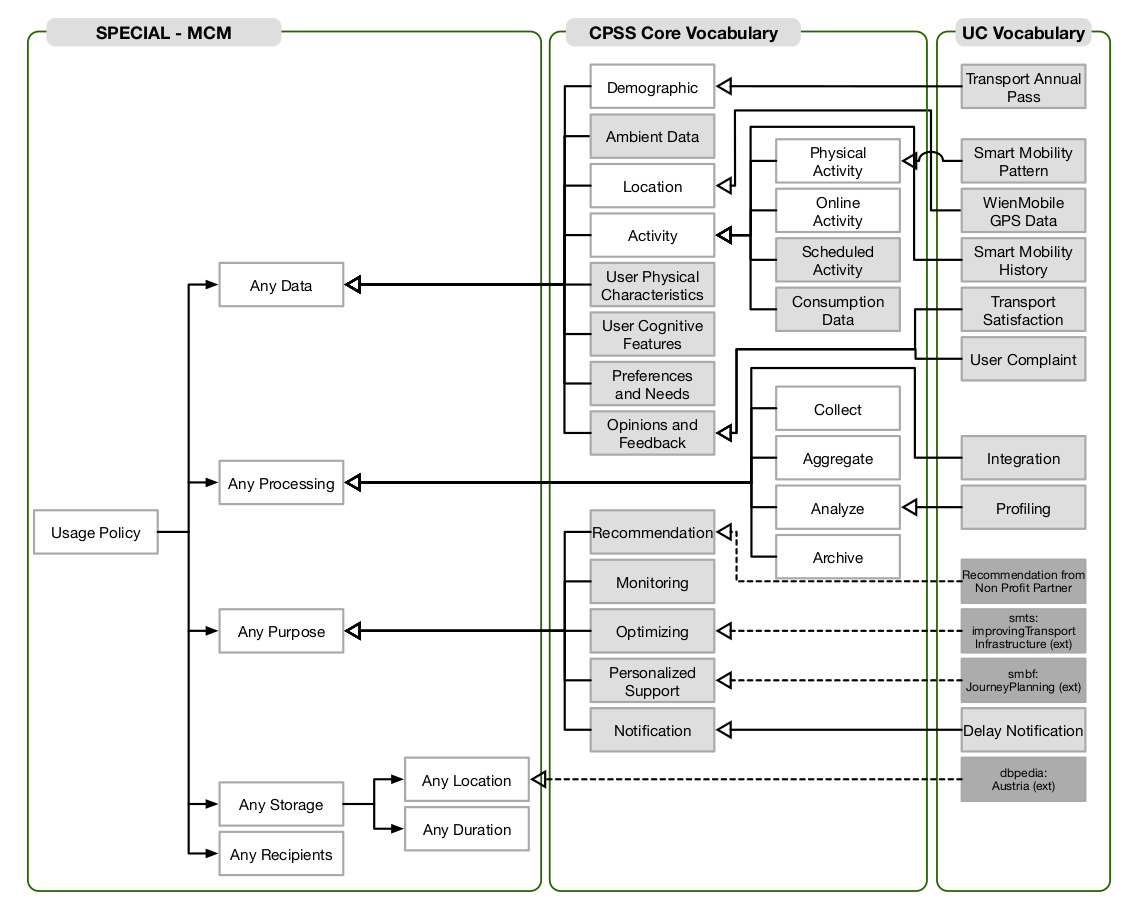
\includegraphics[width=\linewidth]{img/SPECIAL_CitySPIN.png}
    \caption{CitySPIN's extension of SPECIAL vocabularies \cite{fernandez_user_2019}}
    \label{fig:SPECIAL-CitySPIN}
\end{figure}

\subsubsection{MIREL}\label{sota:projects:MIREL}
MIREL\footnote{\url{www.mirelproject.eu/}} (Mining and Reasoning with Legal Texts) is an European H2020 Project that aims to create a framework for interpretation of legal texts into formal representations for querying norms, checking compliance, and decision support. The project uses semantic web to provide normative requirements \cite{gandon_normative_2017}, provide natural language processing over legal texts \cite{milagro_teruel_legal_2018}, and creating ontologies based on GDPR \cite{monica_legal_2018} for legal compliance \cite{palmirani_pronto:_2018-1} and reasoning \cite{palmirani_pronto:_2018}. The project also involves creation of icons for data protection based on the developed ontologies \cite{arianna_dapis:_2019}.
Information about the project is available through peer-reviewed publications and public deliverables\footnote{\url{http://www.mirelproject.eu/publications.php}}.
Details about the project and its developed resources, namely PrOnto, have  been described in publications, but are not open or publicly accessible at the time of writing this thesis.

The developed ontology is termed PrOnto (Privacy Ontology) \cite{monica_legal_2018}, and provides concepts within the GDPR associated with data types and documents, agents and roles, processing purposes, legal bases, processing operations, and deontic operations for modelling rights and duties. It reuses existing vocabularies \cite{palmirani_pronto:_2018} and has been applied within the Cloud4EU project\footnote{\url{http://www.agid.gov.it/cloudforeurope}} for legal compliance checking of eGovernment systems as well as the DAPRECO project (see \autoref{sota:projects:DAPRECO}).

% TODO: diagrams
PrOnto consists of modules representing (i) documents and data, (ii) actors and roles, (iii) processing and workflow, (iv) legal rules and deontic formula, (v) purposes and legal bases. It also includes modules for risk analysis and measures, which it utilises to represent risk management processes such as DPIA as workflows \cite{palmirani_pronto:_2018}. Reasoning is utilised based on the deontic operators within the ontology, and violations are connected with the violated obligations thereby providing traceability towards the steps that created the violation.  LegalRuleML is extended and used to represent the obligations and enable creation and rules for compliance.

% TODO: references
An proof-of-concept application for detecting violations of the GDPR \cite{monica_modelling_2018} utilises PrOnto to model the legal concepts, along with Akoma Ntoso to model the legal text, LegalRuleML to model norms, and Regorous to apply LegalRuleML rules over BPMN and generate a report. The application utlises a web editor for modelling legal rules in connection with the legal text and ontology.

\subsubsection{DAPRECO}\label{sota:projects:DAPRECO}
DAPRECO\footnote{\url{https://www.fnr.lu/projects/data-protection-regulation-compliance/}} (Data Protection Regulation Compliance) is an Luxembourgish project relating to the creation of a knowledge base for formal compliance with the terms and provisions of the GDPR. It aims to provide formalisms in deontic logic and natural language semantics for handling legal norms in written language. The project has researched correlation of standards with laws \cite{bartolini_towards_2016}, creation of an ontology to model concepts in the GDPR \cite{otake_using_2017}, modelling the norms of the GDPR using logic formalisms \cite{bartolini_legal_2018}, and annotating BPMN for GDPR compliance \cite{bartolini_enhancing_2019}.
The project involves collaborations with the MIREL project (see \autoref{sota:projects:MIREL}), particularly in the creation and utilisation of PrOnto for addressing GDPR \cite{monica_legal_2018,palmirani_pronto:_2018,palmirani_pronto:_2018-1,bartolini_enhancing_2019}. In turn, DAPRECO provides a practical application of PrOnto as an use-case for legal compliance over business activities \cite{bartolini_enhancing_2019,bartolini_agile_2019}.

While PrOnto represents a more mature and progressive deliverable of the project's ontology for GDPR, the earlier ontology - referred to as data protection ontology \cite{otake_using_2017} - is relevant for its modelling of the concepts and norms based on an draft of the GDPR. This ontology uses OWL2 to model the concepts of the GDPR and was specified to be a work in progress in its publication\footnote{It can be assumed the ontology is no longer being used or developed and was utilised in the development of PrOnto based on subsequent publications of the project \cite{bartolini_legal_2018,bartolini_enhancing_2019}.}. The ontology can be accessed publicly\footnote{Link from \cite{otake_using_2017} \url{https://github.com/guerret/lu.uni.eclipse.bpmn2}} with documentation provided using LODE ontology documentation tool \cite{peroni_tools_2013}.

Subsequent applications of PrOnto in the project utilises Reified Input/Output logic (RIO) \cite{robaldo_reified_2017} - a formalism for normative reasoning based on reification applied to natural language semantics. The rules are expressed using LegalRuleML and are associated with activities using BPMN. This is utilised to allocate tasks related to data protection to stakeholders, and to track compliance across different phases of a software development life-cycle.

% non sem-web
\subsubsection{My Health My Data (MHMD)}
My Health My Data\footnote{\url{http://www.myhealthmydata.eu/}} (MHMD) is an European H2020 project that aims to develop infrastructure based on blockchain and smart contracts, which provide personal data accounts in the cloud that can be managed using dynamic consent interfaces and provide peer-to-peer connections between stakeholders. The project uses blockchain to log data transactions in a secure, transparent, and accountable manner, while using de-identification and encryption to protect identity and sensitive information. The safety and security of the data is tested using re-identification and penetration simulations.
Information about the project is available through peer-reviewed publications and public deliverables\footnote{\url{http://www.myhealthmydata.eu/publicdeliverables/}}.

The project is applied over the use-case of health data and devices, described in deliverable D1.1 \cite{noauthor_d1.1_initial-list--main-requirements.pdf_nodate}, and uses an ontological resource to model the common data ontology - described more in its deliverable D4.2 \cite{teodoro_d4.2-mhmd-ontological-resources.pdf_2018}. The common data ontology consists of modular health data ontologies representing synthetic data shared by the project's commercial partners as an use-case.
Access to the data is provided through an API that includes parameters describing the requested data category as well as consent descriptions. The API returns matching datasets which can then be utilised for data processing activities. The consent description parameter of the API is a text field consisting of values such as ``synthetic data'' and ``fully anonymised'' which reflect the state of data and its requirements in terms of consent. 

Though the project aims to utilise the GDPR as a source of legal requirements and strives to design its framework to meet compliance requirements by both design and default, there is no publicly available information regarding the specifics of how GDPR compliance is achieved or represented.
It focuses on the privacy preserving and security aspects of data storage by using technological solutions such as access control and transparent logging to design specifications based on legal requirements.
The project does explores the impact of GDPR of storing data in a blockchain, especially regarding the right to be forgotten \cite{bayle_when_2018}.

\subsubsection{RestAssured}

6> BPR4GDPR

7> DEFEND

8> Papaya

9> SMOOTH

10> STAR

0> Other Projects
- SODA
- DECODE 
- MOSAICrOWN
- MUSKETEER
- OPERANDO
- PDP4E
-PoSEID-on
- PRIPARE
- 

\subsection{Research Approaches utilising Semantic Web}

\section{Other Approaches for GDPR compliance}\label{sec:sota:gdpr-other}

\section{Other Relevant Approaches for Legal Compliance}\label{sec:sota:other}

\section{Analysis \& Discussion}\label{sec:sota:analysis}